%% LaTeX2e class for student theses
%% sections/evaluation.tex
%% 
%% Karlsruhe Institute of Technology
%% Institute for Program Structures and Data Organization
%% Chair for Software Design and Quality (SDQ)
%%
%% Dr.-Ing. Erik Burger
%% burger@kit.edu
%%
%% Version 1.3.3, 2018-04-17

\chapter{Evaluation}
\label{ch:Evaluation}
Das Hauptziel dieser Masterarbeit ist es eine Modellierung einer MOM mit expliziten Warteschlangen zu ermöglichen und anschließend in Performance-Analysen zu untersuchen. Um dieses Ziel zu erreichen wurde in \autoref{ch:modellierung} eine Modellierungsmethode vorgestellt mit der eine MOM modelliert und kalibriert werden kann. Die in \autoref{ch:mom} ausgemessenen Ergebnisse wurden dabei zum Kalibrieren der Modelle verwendet. Im Folgenden, soll die bisherige Arbeit evaluiert werden und dabei gezeigt werden, dass die definierten Ziele erreicht werden konnten. 

Die Ziele und die Bewertung, ob diese erreicht werden konnten werden mithilfe der Goal-Question-Metric (GQM) untersucht.
Die GQM-Methode \cite{gqm} spezifiziert Ziele für das zu evaluierende Konzept. Daraufhin werden zu den Zielen Fragen spezifiziert, mit denen die Erfüllung des Ziels überprüft werden soll. Schließlich werden Metriken festgelegt, durch die die Fragen beantwortet werden sollen. Aus \autoref{tab:gqm} können die Ziele, Fragen und Metriken entnommen werden, mit denen diese Masterarbeit evaluiert werden soll.

Ein Ziel, das mithilfe dieser Masterarbeit erreicht werden soll, ist die Modellierung von MOMs in Palladio zu ermöglichen. Dafür wurden zwei Fragen definiert. Die erste Frage prüft ob sich MOMs überhaupt modellieren lassen. Die zweite Frage prüft die Modularität der MOM Bausteine. Das zweite Ziel ist, dass die Entscheidungsfindung, welche MOM verwendet werden soll, bereits zur Modellierungszeit und aus Architekturperspektive verbessert werden soll. Die dazu definierte Frage soll prüfen ob die Analyseergebnisse brauchbar, bzw. ob sich die Probleme einer Architekturentscheidung aus den Analyseergebnissen ableiten lassen. 
\begin{table}
  \begin{tabular}{|l|l|}
    \hline
    \multicolumn{2}{|l|}{Ziel 1} \\
    \hline
    Zweck & Ermögliche \\
    Qualitätskriterium & eine wartbare und wiederverwendbare Möglichkeit  \\ 
    Prozess & eine MOM zu modellieren \\
    Sicht & aus Architekturperspektive \\
   
    \hline \hline
    Frage 1 & Lassen sich MOMs modellieren? \\
    \hline
    Metrik & - Wie viele MOM Parameter konnten nicht modelliert werden? \\
    & - Wie viele Schritte müssen durchgeführt werden um eine neue \\
    & MOM zu modellieren\\
    \hline\hline
    Frage 2 & Wie modular sind die MOM Bausteine? \\
    \hline
    Metrik & - Wie viele Elemente müssen beim Austausch geändert werden? \\
    & - Min. Anzahl an Schritte um MOM auszutauschen \\
    \hline\hline
    \multicolumn{2}{|l|}{Ziel 2} \\
    \hline
    Zweck & Verbessere \\
    Qualitätskriterium & die Abwägung und Entscheidungsfindung  \\ 
    Prozess & beim Einsatz einer MOM \\
    Sicht & aus Architekturperspektive \\
    \hline \hline
    Frage 1 & Sind die Analyse Ergebnisse brauchbar? \\
    \hline
    Metrik & - Wie viel \% Abweichung zur naiven Modellierung/Implementierung? \\
    & - Wie viele Schritte müssen durchgeführt werden um Problem der \\
    & Architekturentscheidung aus dem Analyseergebnis abzuleiten? \\
    \hline
  \end{tabular}
	\caption{\label{tab:gqm} Ziele, Fragen und Metriken für die Evaluierung, nach der GQM-Methode}
\end{table}


%\section{Systemanforderungen}
%\label{sec:systemanforderungen}
%Für das Evaluierungssystem wurden im Folgenden Anforderungen festgelegt.
%\begin{itemize}
%\item Das jeweilige System soll \textbf{Skalierung} erlauben. Dabei soll es zum einen möglich sein die Anzahl von Kommunikationspartnern zu erhöhen (\textit{horizontal}) als auch die Menge an Nachrichten die verschickt werden (\textit{vertikal}).
%\item Weitere \textbf{Konfigurationen} wie Nachrichtengröße, reihenfolgentreue, Duplikate, etc. sollten möglich sein.
%\item System soll möglichst \textbf{reales System} darstellen.
%\item Mindestens ein \textbf{Nachrichtenmodell} sollte unterstützt werden.
%\item Es sollten \textbf{verschiedene Interaktionstypen} unterstützt werden, wie Many-To-Many, Many-To-One, etc.
%\item Damit der Fokus der Masterarbeit auf den MOMs und ihrer Modellierung liegt, sollte das System \textbf{bereits vorhanden} und implementiert und modelliert sein.
%\end{itemize}

\section{SPECJms2007}
Das für die Evaluierung verwendete System ist das im SPECJms2007 Benchmark verwendete Testsystem \cite{Sachs2013}. Der Benchmark stellt eine reale ereignisbasierte Anwendung dar und umfasst eine Reihe von verschiedener Interaktionen, die sowohl Punkt-zu-Punkt- als auch Publish/Subscribe-Nachrichten einschließlich One-to-One-, One-to-Many- und Many-to-Many-Kommunikation umfasst. Das Hauptziel des SPECjms2007 Benchmarks ist es, einen Standard-Workload bereitzustellen, der die Leistung und Skalierbarkeit von JMS-basierten Message-Oriented Middleware-Plattformen bewertet. Bei dem System handelt es sich um ein Lieferkettenmanagement für eine Supermarktkette. Der Benchmark verwendet verschiedene Nachrichtentypen und verwendet Nachrichten verschiedenen Größe. Für die Masterarbeit liegt sowohl die Implementierung des Benchmarks, als auch eine Modellierung aus einer früheren Arbeit von Christoph Rathfelder \cite{Rathfelder2013} vor. Dieses System soll als Experimentsystem verwendet werden um die verschiedenen MOMs zu vergleichen und zum kalibrieren der später erstellten Modellierung. 

\subsection{Anwendungsszenario}
Das gewählte Anwendungsszenario bildet die Lieferkette eines Supermarktunternehmens ab. In \autoref{img:specjmsInteraction} sind die beteiligten Rollen abgebildet und wie sie miteinander kommunizieren. Die beteiligten lassen sich wie folgt gruppieren: 
\begin{itemize}
    \item Hauptquartier (HQ): Für die Buchhaltung des Unternehmens verantwortlich. Beobachtet den Geld und Warenfluss im System. Verwaltet Informationen ueber Waren und definiert Preise.
    \item Supermarkt (SM): Verkauft Waren an Kunden. Im Benchmark liegt der Fokus auf der Verwaltung der eigenen Warenlager. Jeder SM ist mit einem Vertriebszentrum verbunden.
    \item Vertriebszentrum (DC): Beliefert SM mit Waren. Ein DC nimmt Aufträge von SMs an und liefert diese. Wenn ein DC die Waren nicht vorrätig hat, werden diese Waren von einem Zulieferer angefordert. Außerdem sind DCs dafür verantwortlich Verkaufsstatistiken an das HQ zu senden.
    \item Zulieferer (SP): SPs sind nicht Teil des Supermarktunternehmens. Jeder SP bietet eine bestimmte Art von Waren an. Diese werden an DCs geliefert, wenn angefordert.
\end{itemize}

\begin{figure}
\center
  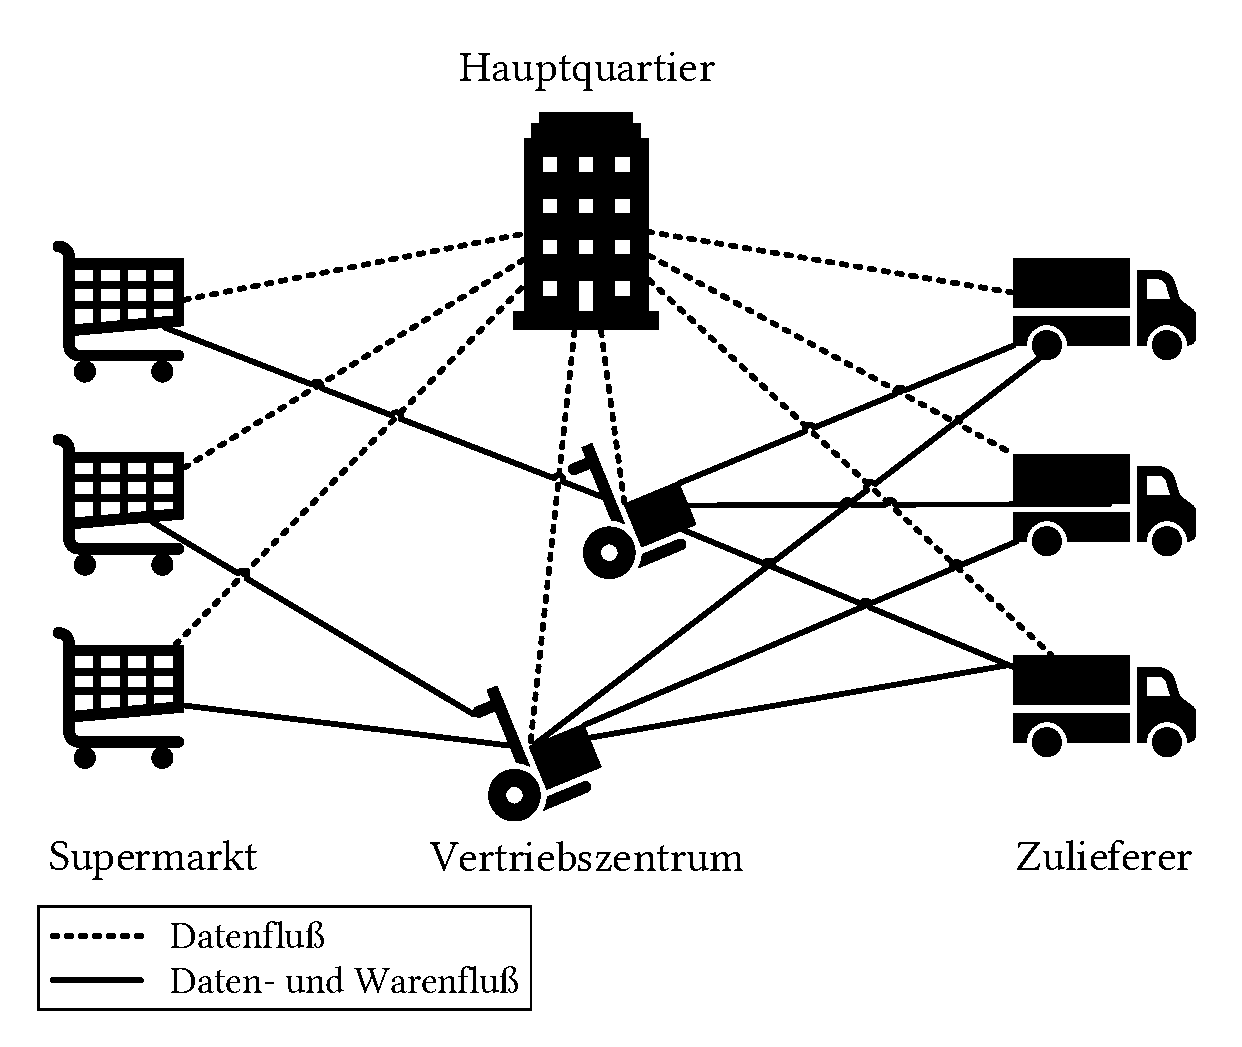
\includegraphics[width=0.7\textwidth]{images/evaluation/specjms/specjmsOverview.pdf}
  \caption{Anwendungszenario des SpecJms}
  \label{img:specjmsInteraction}
\end{figure}

\subsection{Interaktionen und Kommunikation}
SpecJms sieht insgesamt sieben verschiedenen Interaktionsmöglichkeiten vor: 
\begin{enumerate}
    \item Bestell- und Versandabwicklung zwischen SM und seinem DC (Punkt-Zu-Punkt).
    \item Bestell- und Versandabwicklung zwischen DC und seinen SPs (Punkt-Zu-Punkt und Publisher/Subsciber).
    \item Preisaktualisierung (Publisher/Subsciber).
    \item Inventurmanagmenet (Punkt-Zu-Punkt).
    \item Verkaufsstatistik Sammlung (Punkt-Zu-Punkt).
    \item Bekanntmachungen zu Produkten (Publisher/Subsciber).
    \item Kreditkarten Hot-List (Publisher/Subsciber).
    
\end{enumerate}
Im Rahmen der Masterarbeit wurden (, aus Zeitlichen Gründen,) zwei dieser Interaktionen betrachtet. Um trotzdem verschiedene Nachrichtenmodelle und Interaktionstypen betrachten zu können wurden die folgenden beiden Interaktionen ausgewählt.
%warum wurden nur 2 und wiese genau diese ausgewaehlt? (Zeit, welche kommunikationsarten konnten abgedeckt werden?)\\
%Nachrichtenmodelle mit einbeziehen \\
%Interaktionstypen mit einbeziehen \\
\subsubsection{Interaktion 1}
Diese Interaktion übt Punkt-Zu-Punkt Kommunikation zwischen einem SM und seinem DC und dem DC und dem HQ aus. Die Interaktion wird ausgelöst, wenn Waren im Lager eines SM aufgebraucht sind. Der SM bestellt bei einem DC Nachschub um seine Waren aufzufüllen. Neben dem SM und DC ist das HQ auch an dieser Interaktion beteiligt. In \autoref{img:specjmsInteraction1} ist der Ablauf als Sequenzdiagramm abgebildet. 
\begin{itemize}
    \item Der SM sendet eine Bestellung an seinen DC (Order).
    \item Der DC sendet eine Bestätigung, über den Eingang der Nachricht zurück an den SM (OrderConf).
    \item Die bestellte Ware wird registriert während sie das Warenlager des DC verlässt (ShipDep).
    \item Der DC sendet Informationen über die Transaktion an HQ (StatInfoOrder).
    \item Die bestellte Ware wurde vom DC an SM gesendet und empfangen (ShipInfo).
    \item Der SM sendet eine Bestätigung über den erhalt der Bestellung an DC (ShipConf)
\end{itemize}
%Zunächst sendet der SM eine Order Nachricht an den DC. Der DC bestätigt dem SM den Eingang der Nachricht. Als nächstes werden die Waren verschickt. Dabei werden sie von einem RFID Leser erfasst. Schließlich sendet der DC Informationen über die Transaktion an das HQ. Sobald die Lieferung beim SM ankommt wird eine Bestätigung an DC gesendet.

\begin{figure}
\center
  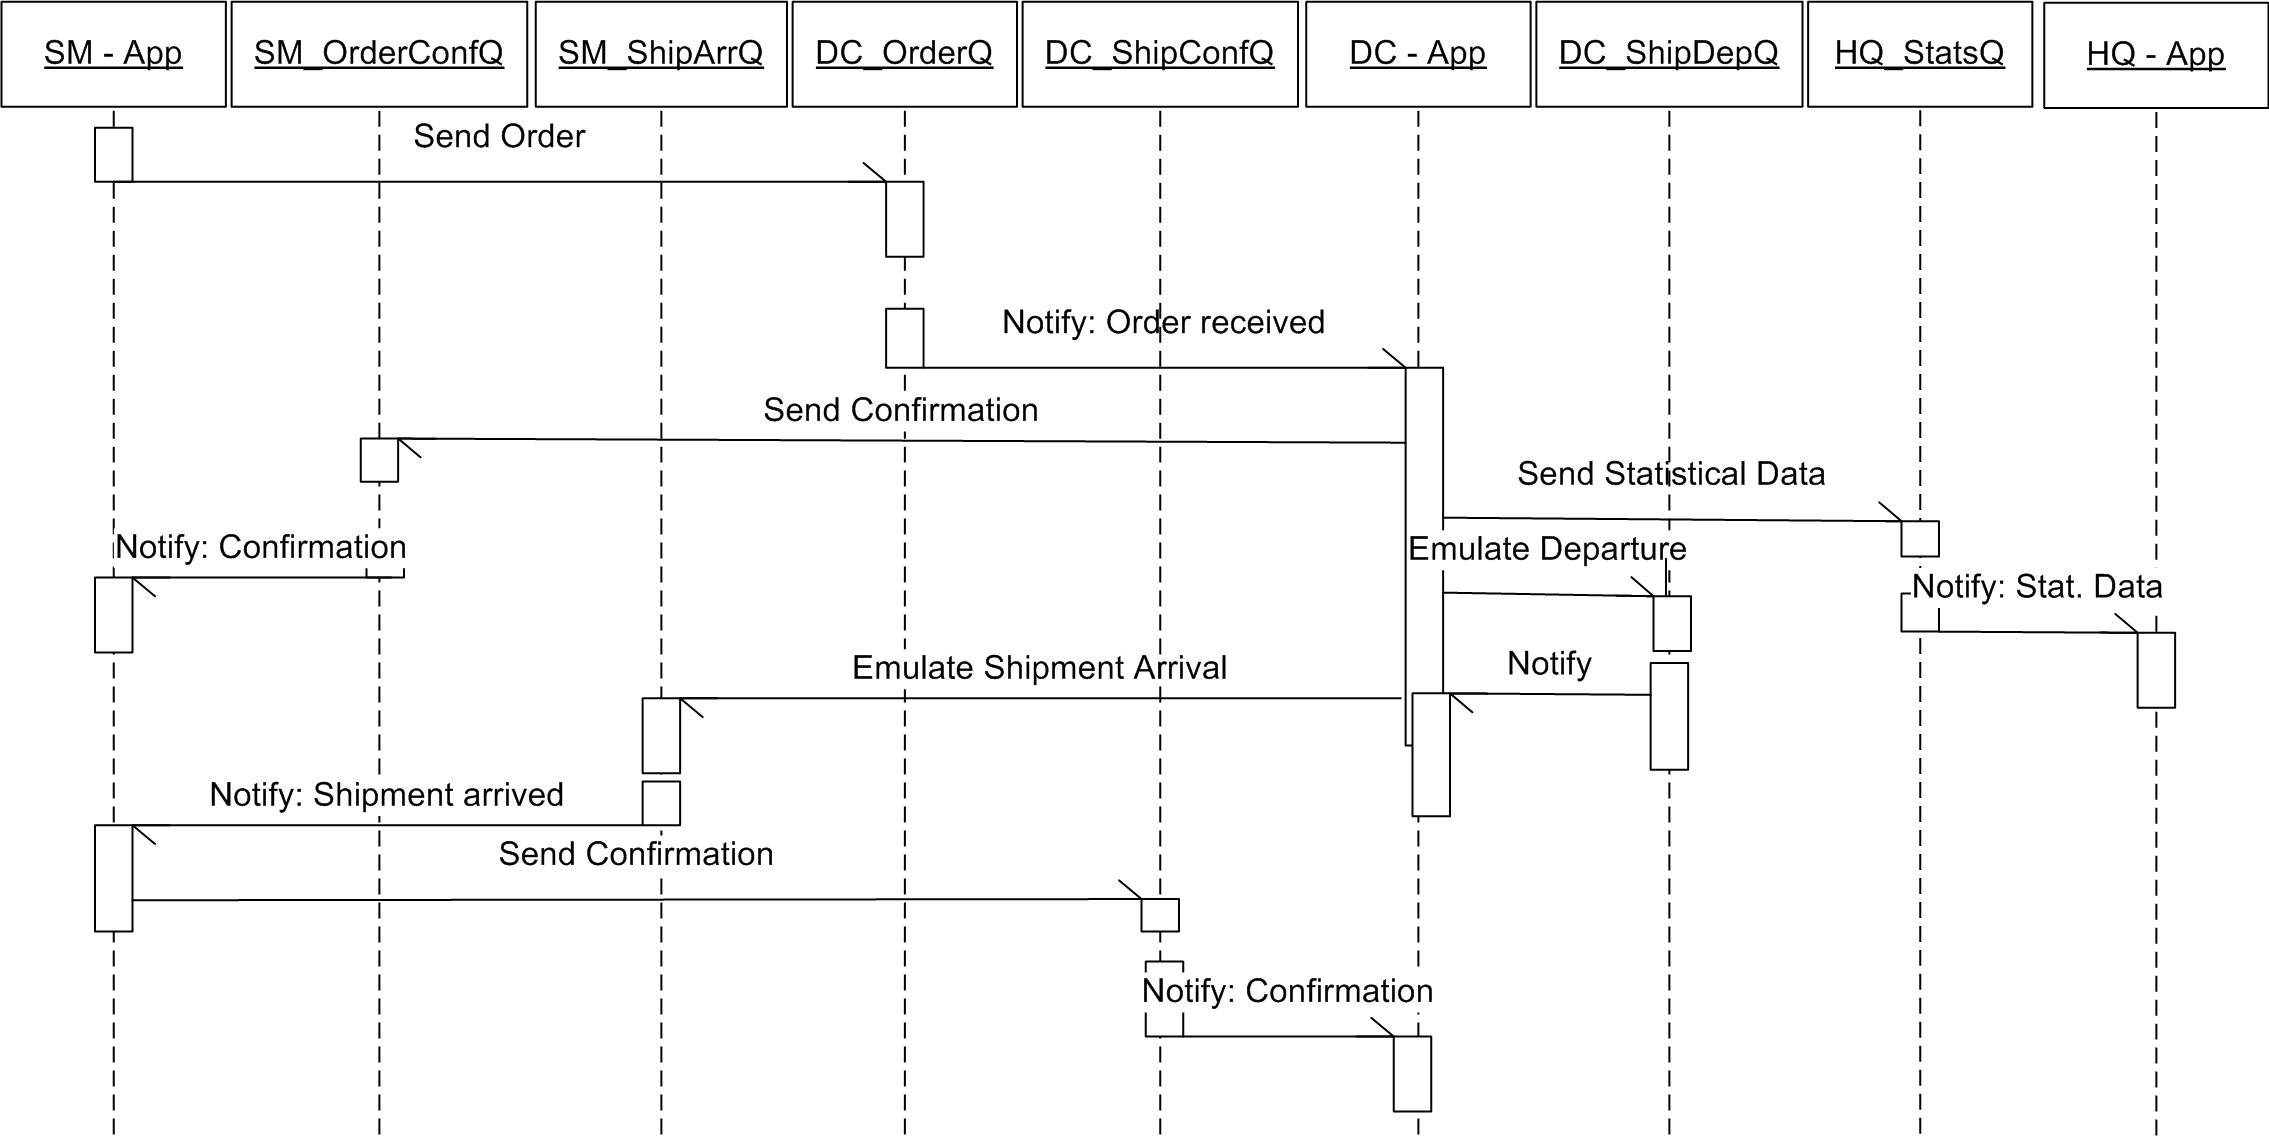
\includegraphics[width=1\textwidth]{images/Interaction1Diag.png}
  \caption{Interaktion 1}
  \label{img:specjmsInteraction1}
\end{figure}

\subsubsection{Interaktion 3}
Diese Interaktion übt Publisher/Subscriber Kommunikation zwischen dem HQ und seinen SMs aus. Es handelt sich um eine Eins-Zu-Viele Kommunikation und wird ausgelöst, wenn die Preise der Ware durch die Firmenleitung (HQ) geändert werden. Um dies zu kommunizieren, sendet das HQ Nachrichten an alle SMs. In \autoref{img:specjmsInteraction3} ist der Ablauf der Interaktion als Sequenzdiagramm abgebildet.
\begin{itemize}
    \item Das HQ sendet ein Preisaktualisierung (PriceUpdate).
    \item Betroffene SMs empfangen und ändern die Information in ihrem System.
\end{itemize}


\begin{figure}
\center
  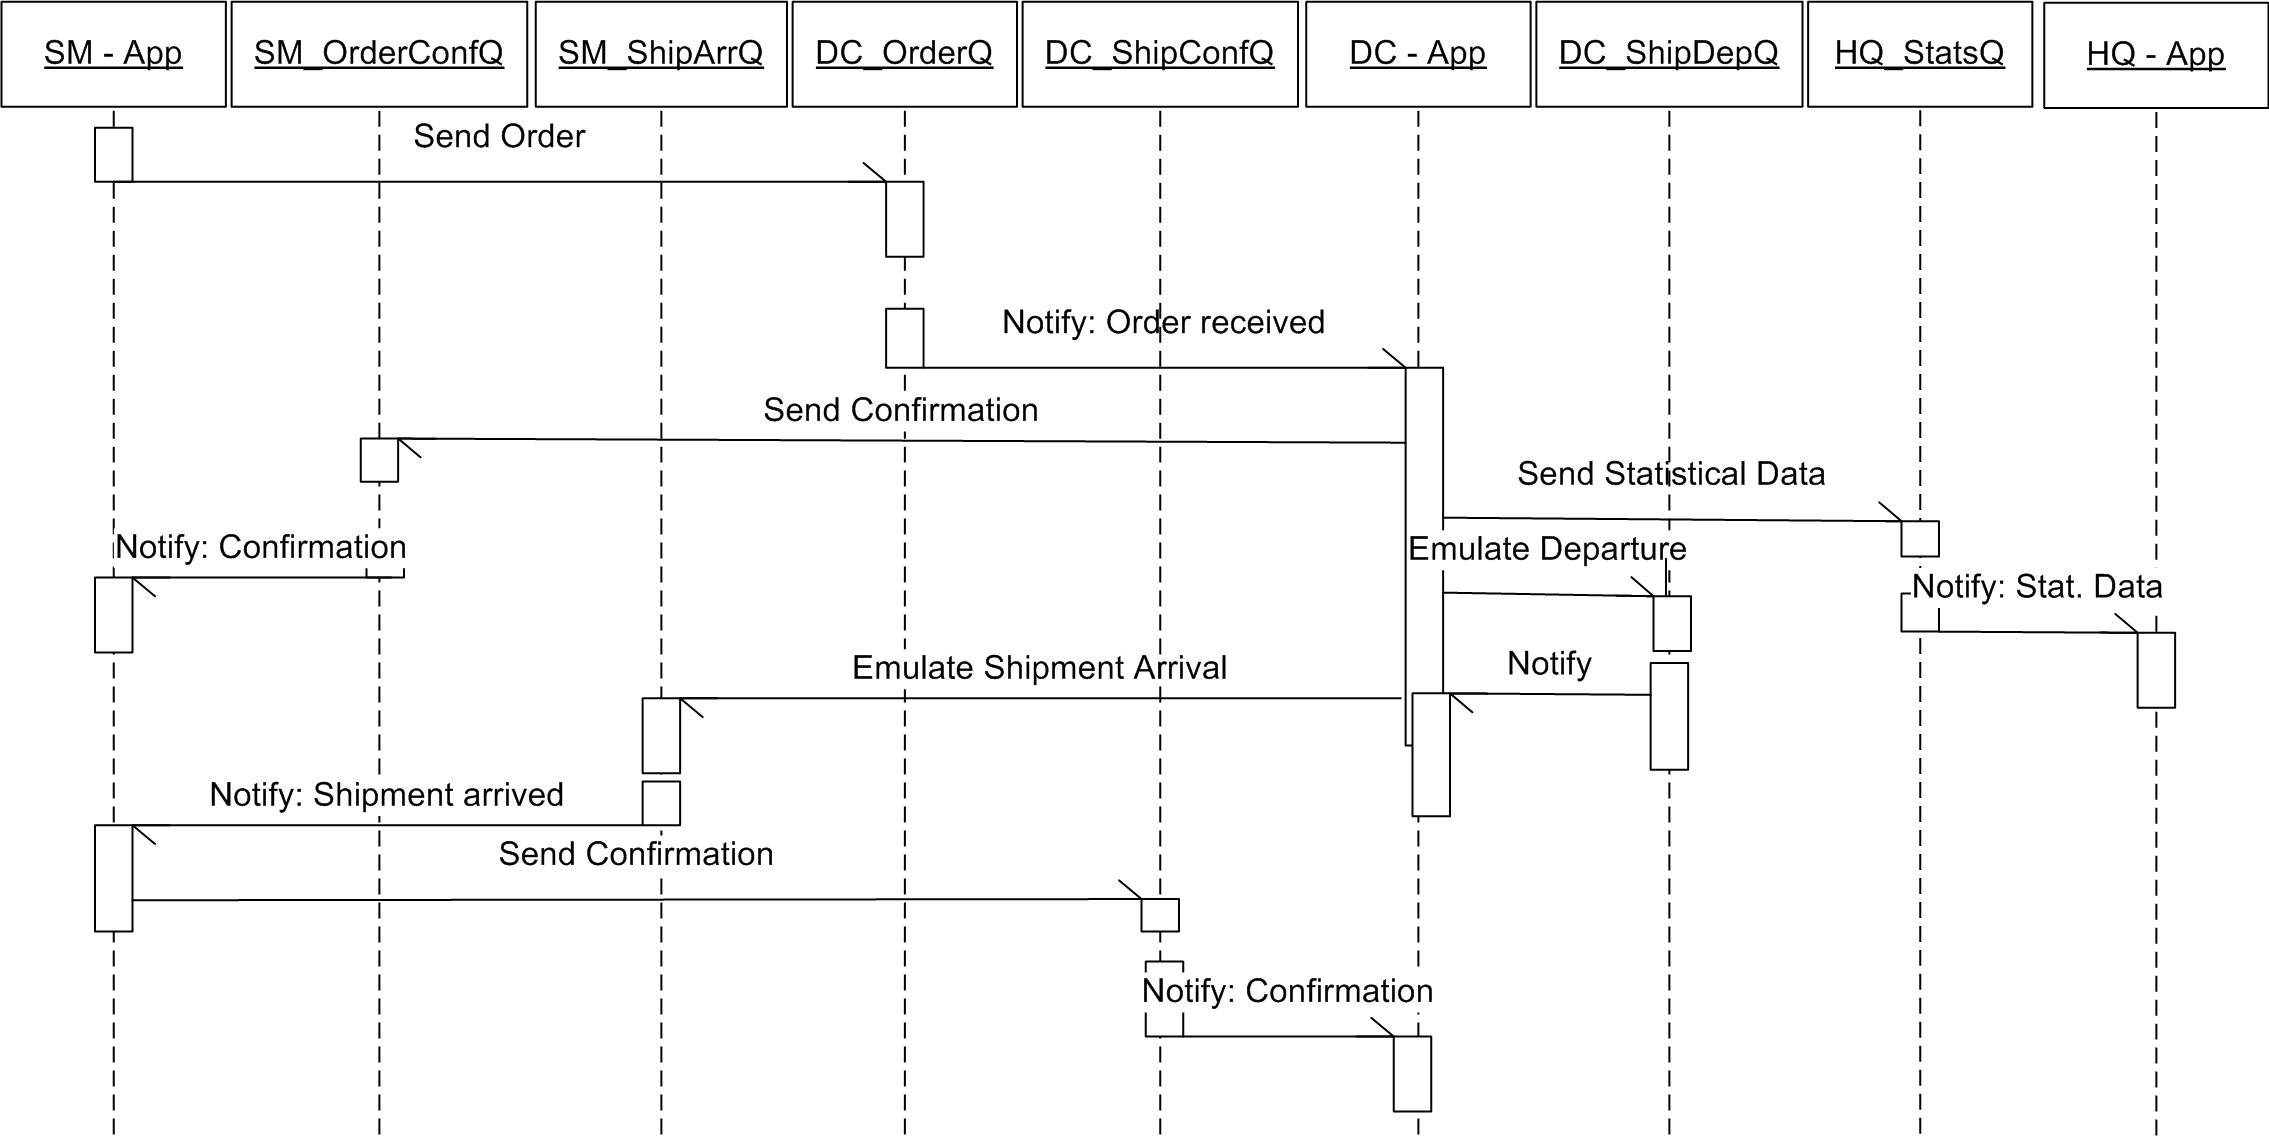
\includegraphics[width=1\textwidth]{images/Interaction1Diag.png}
  \caption{Interaktion 1}
  \label{img:specjmsInteraction3}
\end{figure}


\subsection{Konfiguration}
SpecJMS2007 erlaubt verschiedene Konfigurationen durch den Benutzer. Dabei kann die Toplogie sowhohl horizontal, als auch vertikal skalliert werden. Bei der horizontalen Skalierung, wird die Anzahl der Akteure erhöht, während die Anzahl der gesendeten Nachrichten pro Akteur gleich bleibt. Die vertikale Topologie erhöht die Anzahl der Nachrichten die die Sender senden. Beide Skalierungsarten werden in einer eigenen Konfigurationsdatei mithilfe des Parameters BASE eingestellt.

Außerdem lassen sich für jede Nachricht die Größe und die Verteilung festlegen, mit welcher Wahrscheinlichkeit eine bestimmte Nachrichtengröße auftritt. Die Nachrichtengröße wird dabei mit folgender Formel berechnet: 
\[m1 + x * b\] 
Dabei kann x vom Benutzer des Benchmarks eingestellt werden. Die beiden anderen Parameter wurden in der Arbeit von Sachs et al.\cite{Sachs2013} hergeleitet. Somit kann für jede Nachricht die Wahrscheinlichkeit und ihre Größe festgelegt werden. In \autoref{tab:parameters} sind die für diese Arbeit wichtigen Parameter abgebildet. Die Verteilungen und die dazugehörige Nachrichtengrößen sind in \autoref{tab:msgpropandsize} abgebildet.


\begin{table}
\center
  \begin{tabular}{|c|l|l|l|}
  \hline
    \textbf{Interaktion} & \textbf{Nachricht} & \textit{m1} & \textit{b}  \\
    \hline \hline
    \multirow{6}{*}{1} & Order & 0,0565 & 1,4534 \\\cline{2-4}
    & OrderConf & 0,0565 & 1,4534 \\\cline{2-4}
    & ShipDep & 0,0787 & 0,7222 \\\cline{2-4}
    & StatInfoOrder & 0,0153 & 0,1463 \\\cline{2-4}
    & ShipInfo & 0,0787 & 0,8912 \\\cline{2-4}
    & ShipConf & 0,0202 & 0,7140  \\\hline
    \hline
     3 & PriceUpdate & - & 2,310 \\\hline
  \end{tabular}
	\caption{\label{tab:parameters} Parameter zur Berechnung der Nachrichtengröße.}
\end{table}

\begin{table}
\center
  \begin{tabular}{|c|l|l|l|l|}
  \hline
    \textbf{Interaktion} & \textbf{Nachricht} & \textbf{Größe 1} & \textbf{Größe 2} &\textbf{Größe 3} \\
     & \textit{Wahrscheinlichkeit} & \textit{95\%}  & \textit{4\%} &\textit{1\%}   \\
    \hline \hline
    \multirow{6}{*}{1} & Order & 1,74 & 7,10 & 41,01 \\\cline{2-5}
    & OrderConf & 2,02 & 7,39 & 41,29 \\\cline{2-5}
    & ShipDep & 1,12 & 8,59 & 55,79\\\cline{2-5}
    & StatInfoOrder & 0,22 & 1,67 & 10,83 \\\cline{2-5}
    & ShipInfo & 1,28 & 8,76 & 55,95 \\\cline{2-5}
    & ShipConf & 0,81 & 2,73 & 14,83  \\\hline
    \hline
     3 & PriceUpdate & 0,24 & 0,24 & 0,24 \\\hline
  \end{tabular}
	\caption{\label{tab:msgpropandsize} Nachrichtengröße in KByte.}
\end{table}

\section{Beschreibung des Modells}
Modelle sind uebernommen worden aus diss. \\
beschreibe Ist zustand inklussive MOM
\subsection{Ist Zustand}
\subsubsection{System}
Direkte Verbindung der Kommunikationen \\
RD innerhalb von Kommunikation (Verarbeitung von Nachrichten, bevor weiter geleitet, etc.)\\
Pub/sub ueber EventChannel \\
Start einer Interaktion wird durch Trigger ausgeloesst \\
Interaktion 1: \autoref{img:interaction1system}

Interaktion 3: \autoref{img:interaction3system}

\begin{figure}
\center
  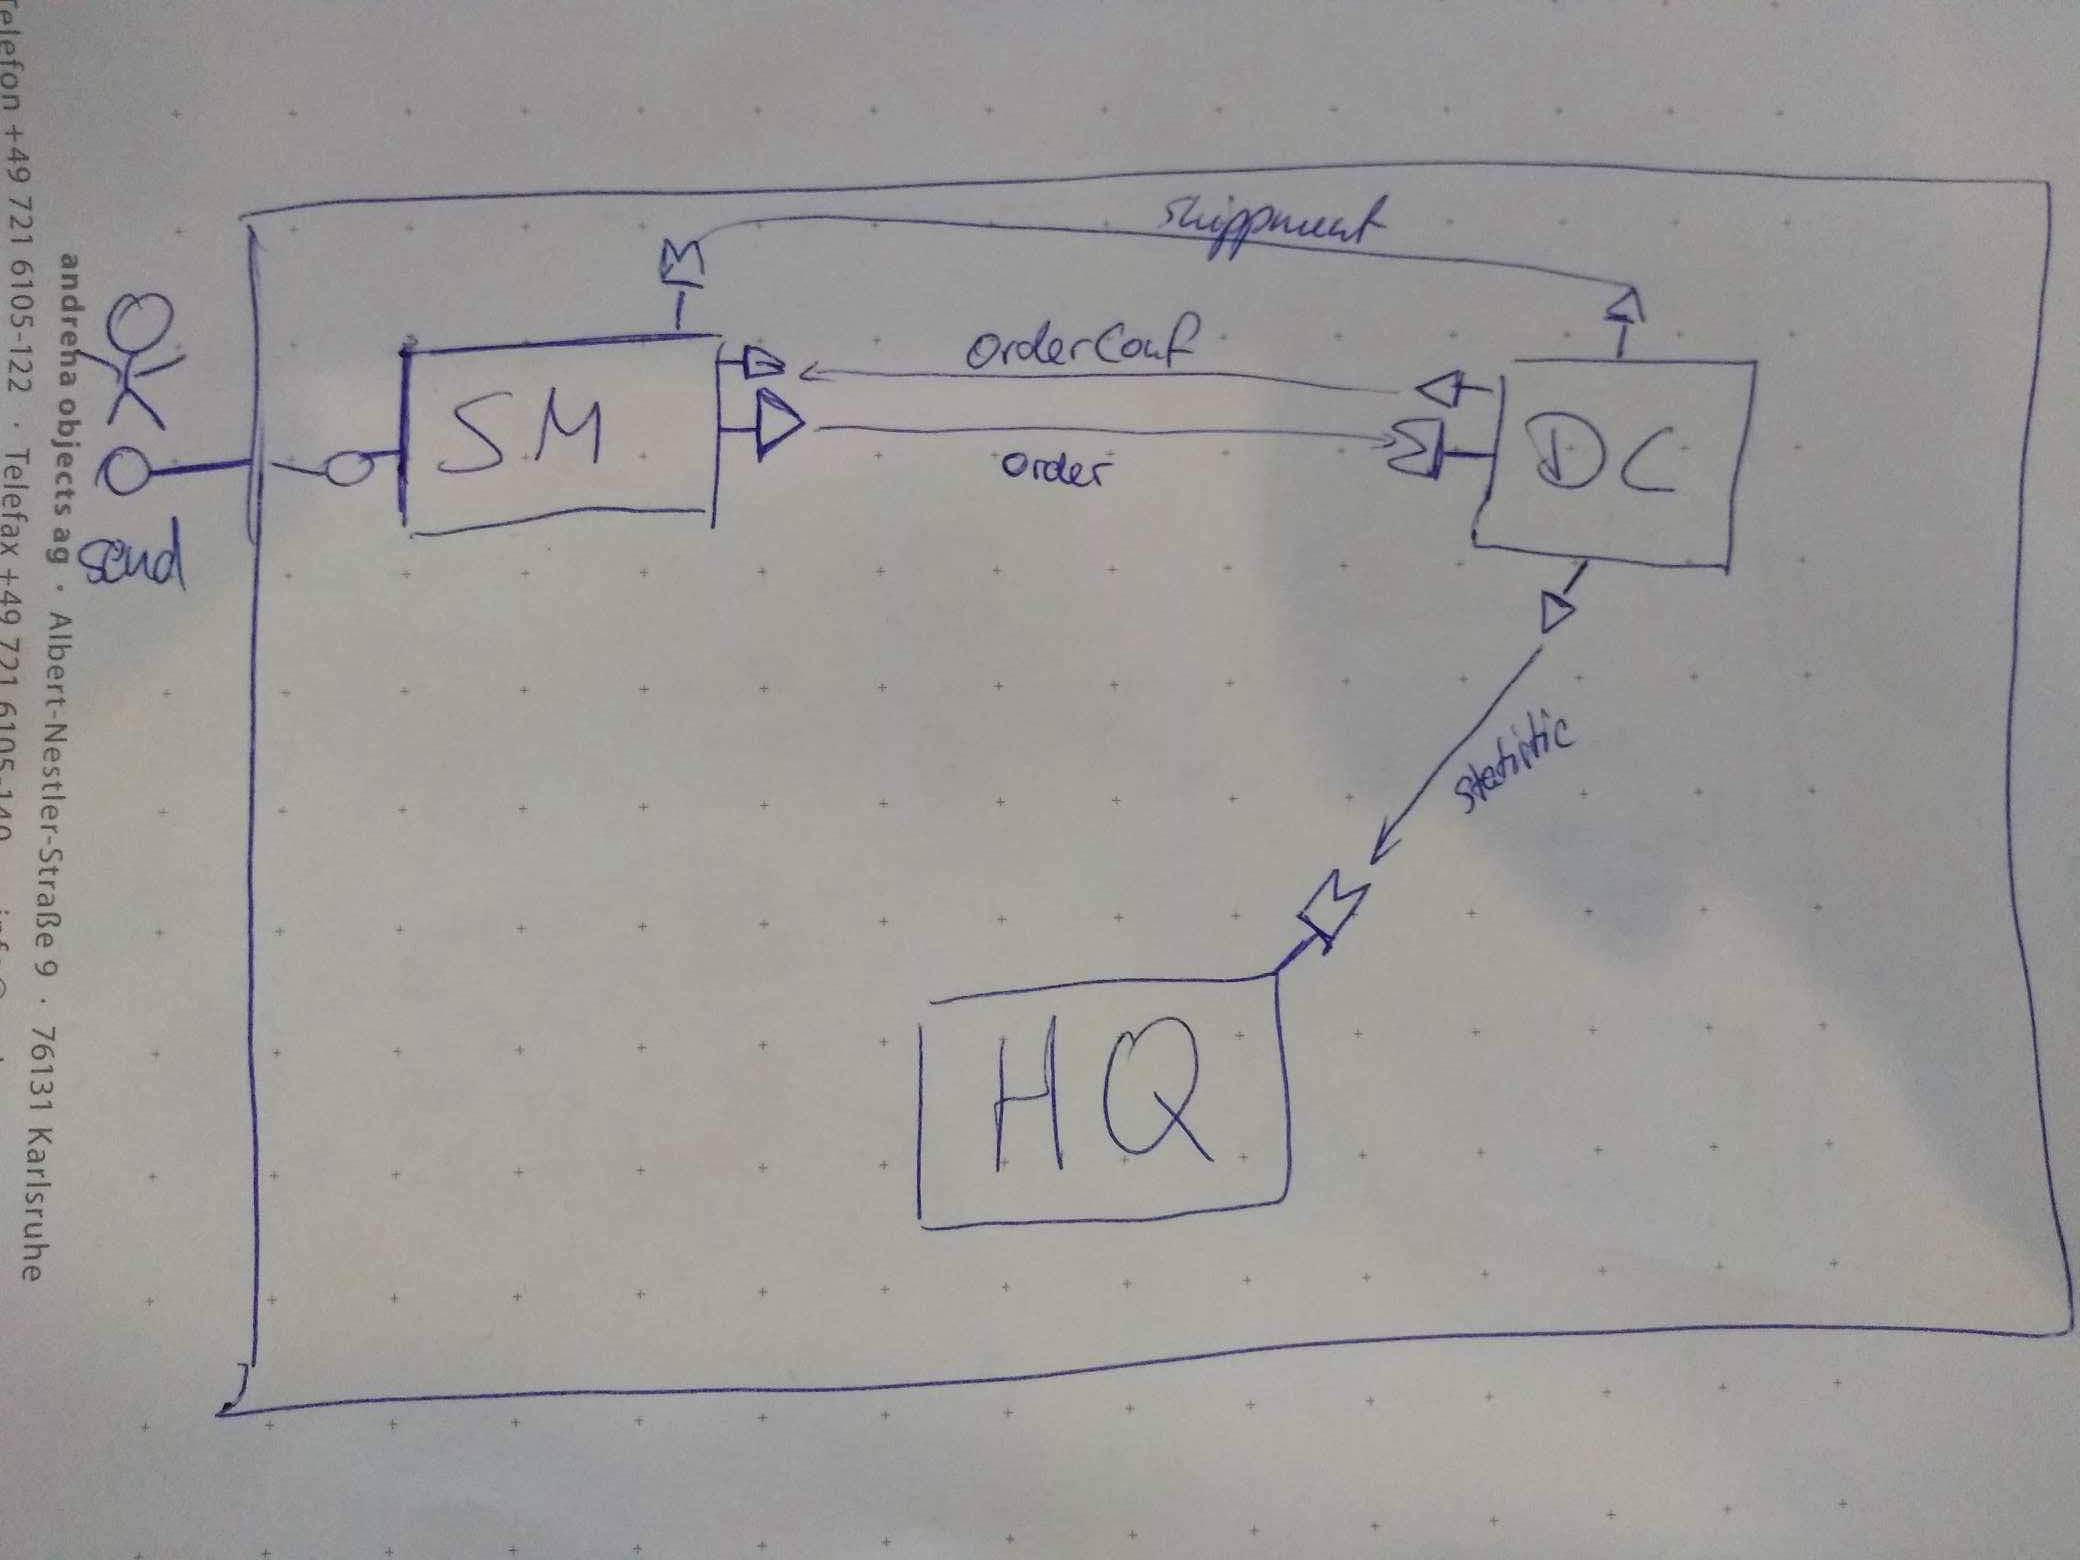
\includegraphics[width=1\textwidth]{images/evaluation/specjms/interaction1system_events.png}
  \caption{Interaktion 1 mit Events}
  \label{img:interaction1system}
\end{figure}

\begin{figure}
\center
  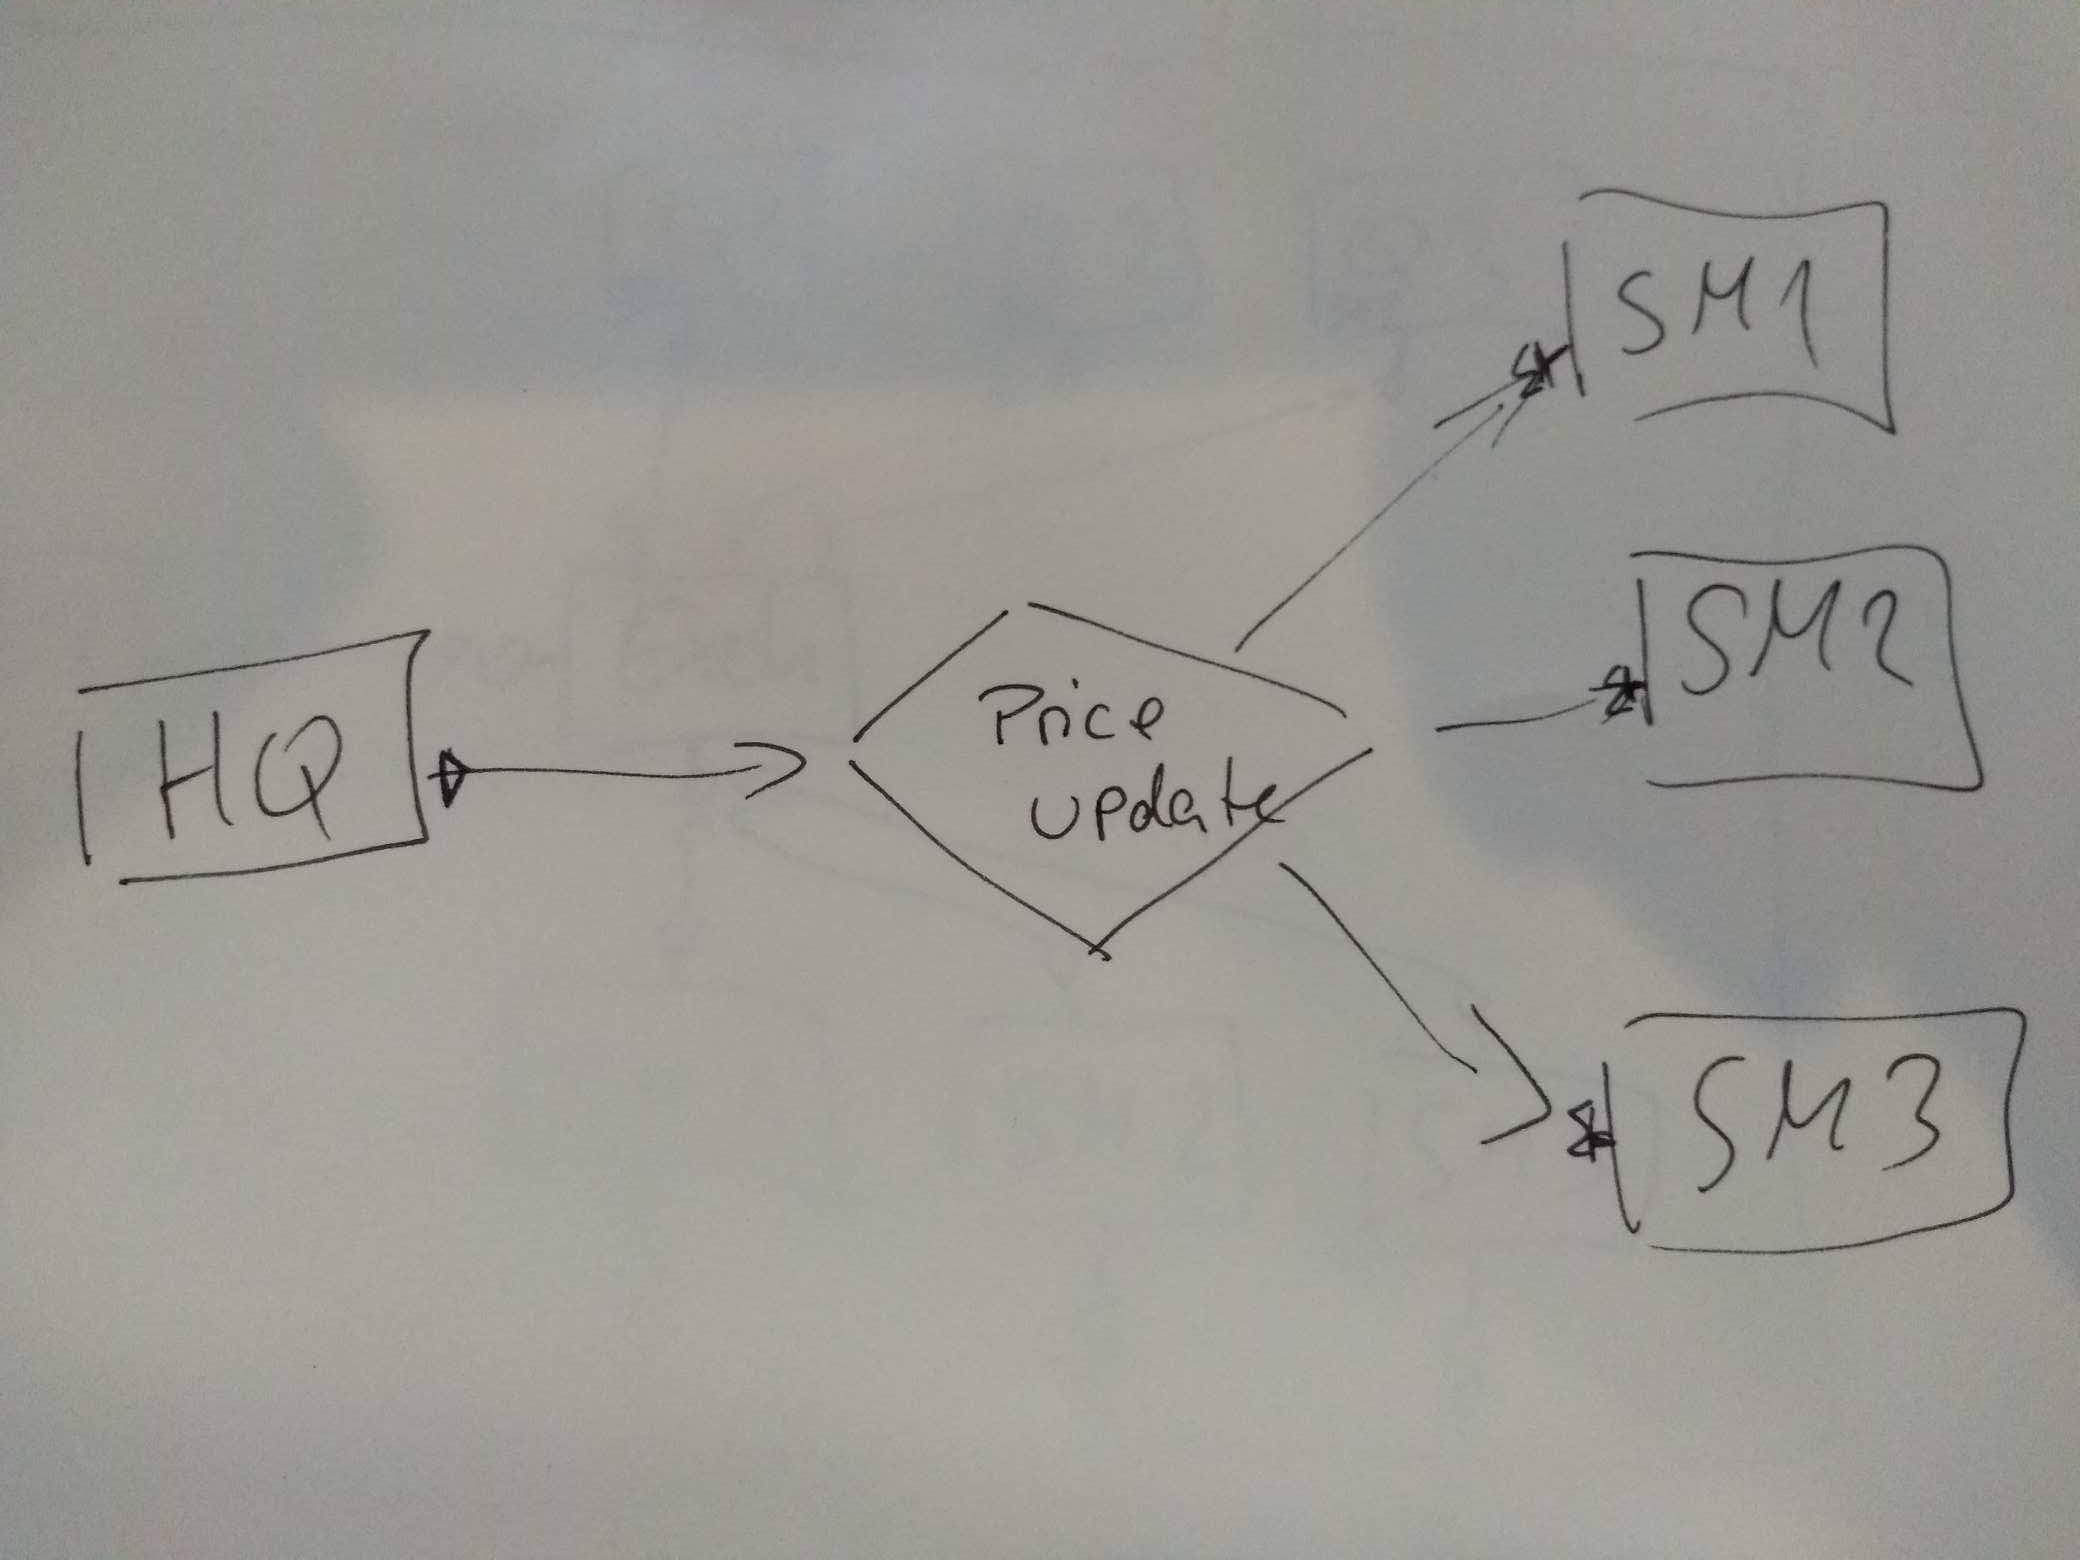
\includegraphics[width=1\textwidth]{images/evaluation/specjms/interaction3system_events.png}
  \caption{Interaktion 3 mit Events}
  \label{img:interaction3system}
\end{figure}
\subsubsection{Ressource und Allocation}
\subsubsection{Usage}
\subsubsection{MOM}
RD fuer jede Moegliche Nachricht angegeben und davor ausgerechnet, siehe \autoref{img:specjmsMsgSizeRd} \\
\begin{figure}
\center
  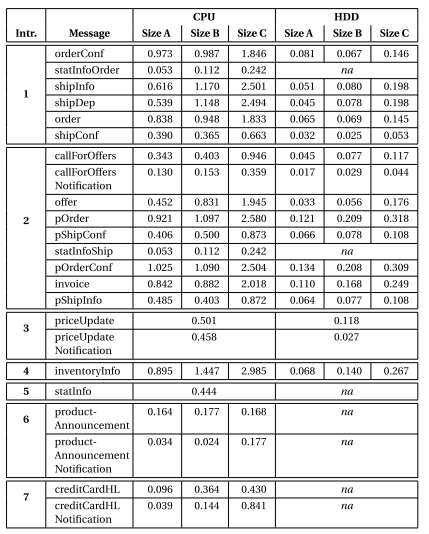
\includegraphics[width=1\textwidth]{images/specjmsmsgsizerd.png}
  \caption{Ausgerechnete RDs fuer jede Nachricht}
  \label{img:specjmsMsgSizeRd}
\end{figure}


\subsection{Anpassung des Modells}
Meine Transformation wird verwendet anstatt Event Transformation \\
MOM Modell wird nicht verwendet\\
msg size wird nicht mehr in MOM fuer jede Nachricht berechnet und eingepflegt, sondern werden im UsageModell oder beim EmitEvent (incl) Verteilung mitgegeben \\

evtl nachrichtengröße wird in usage modell mit angegeben \\
nachrichtengröße mit verteilung angegeben und nicht verteilung und rd


\subsection{Modell nach Transformation}
Beschreibe Modelle nach Transformation \\
\subsubsection{Interaktion 1}
\autoref{img:interaction1systemAfterTransformation}
\begin{figure}
\center
  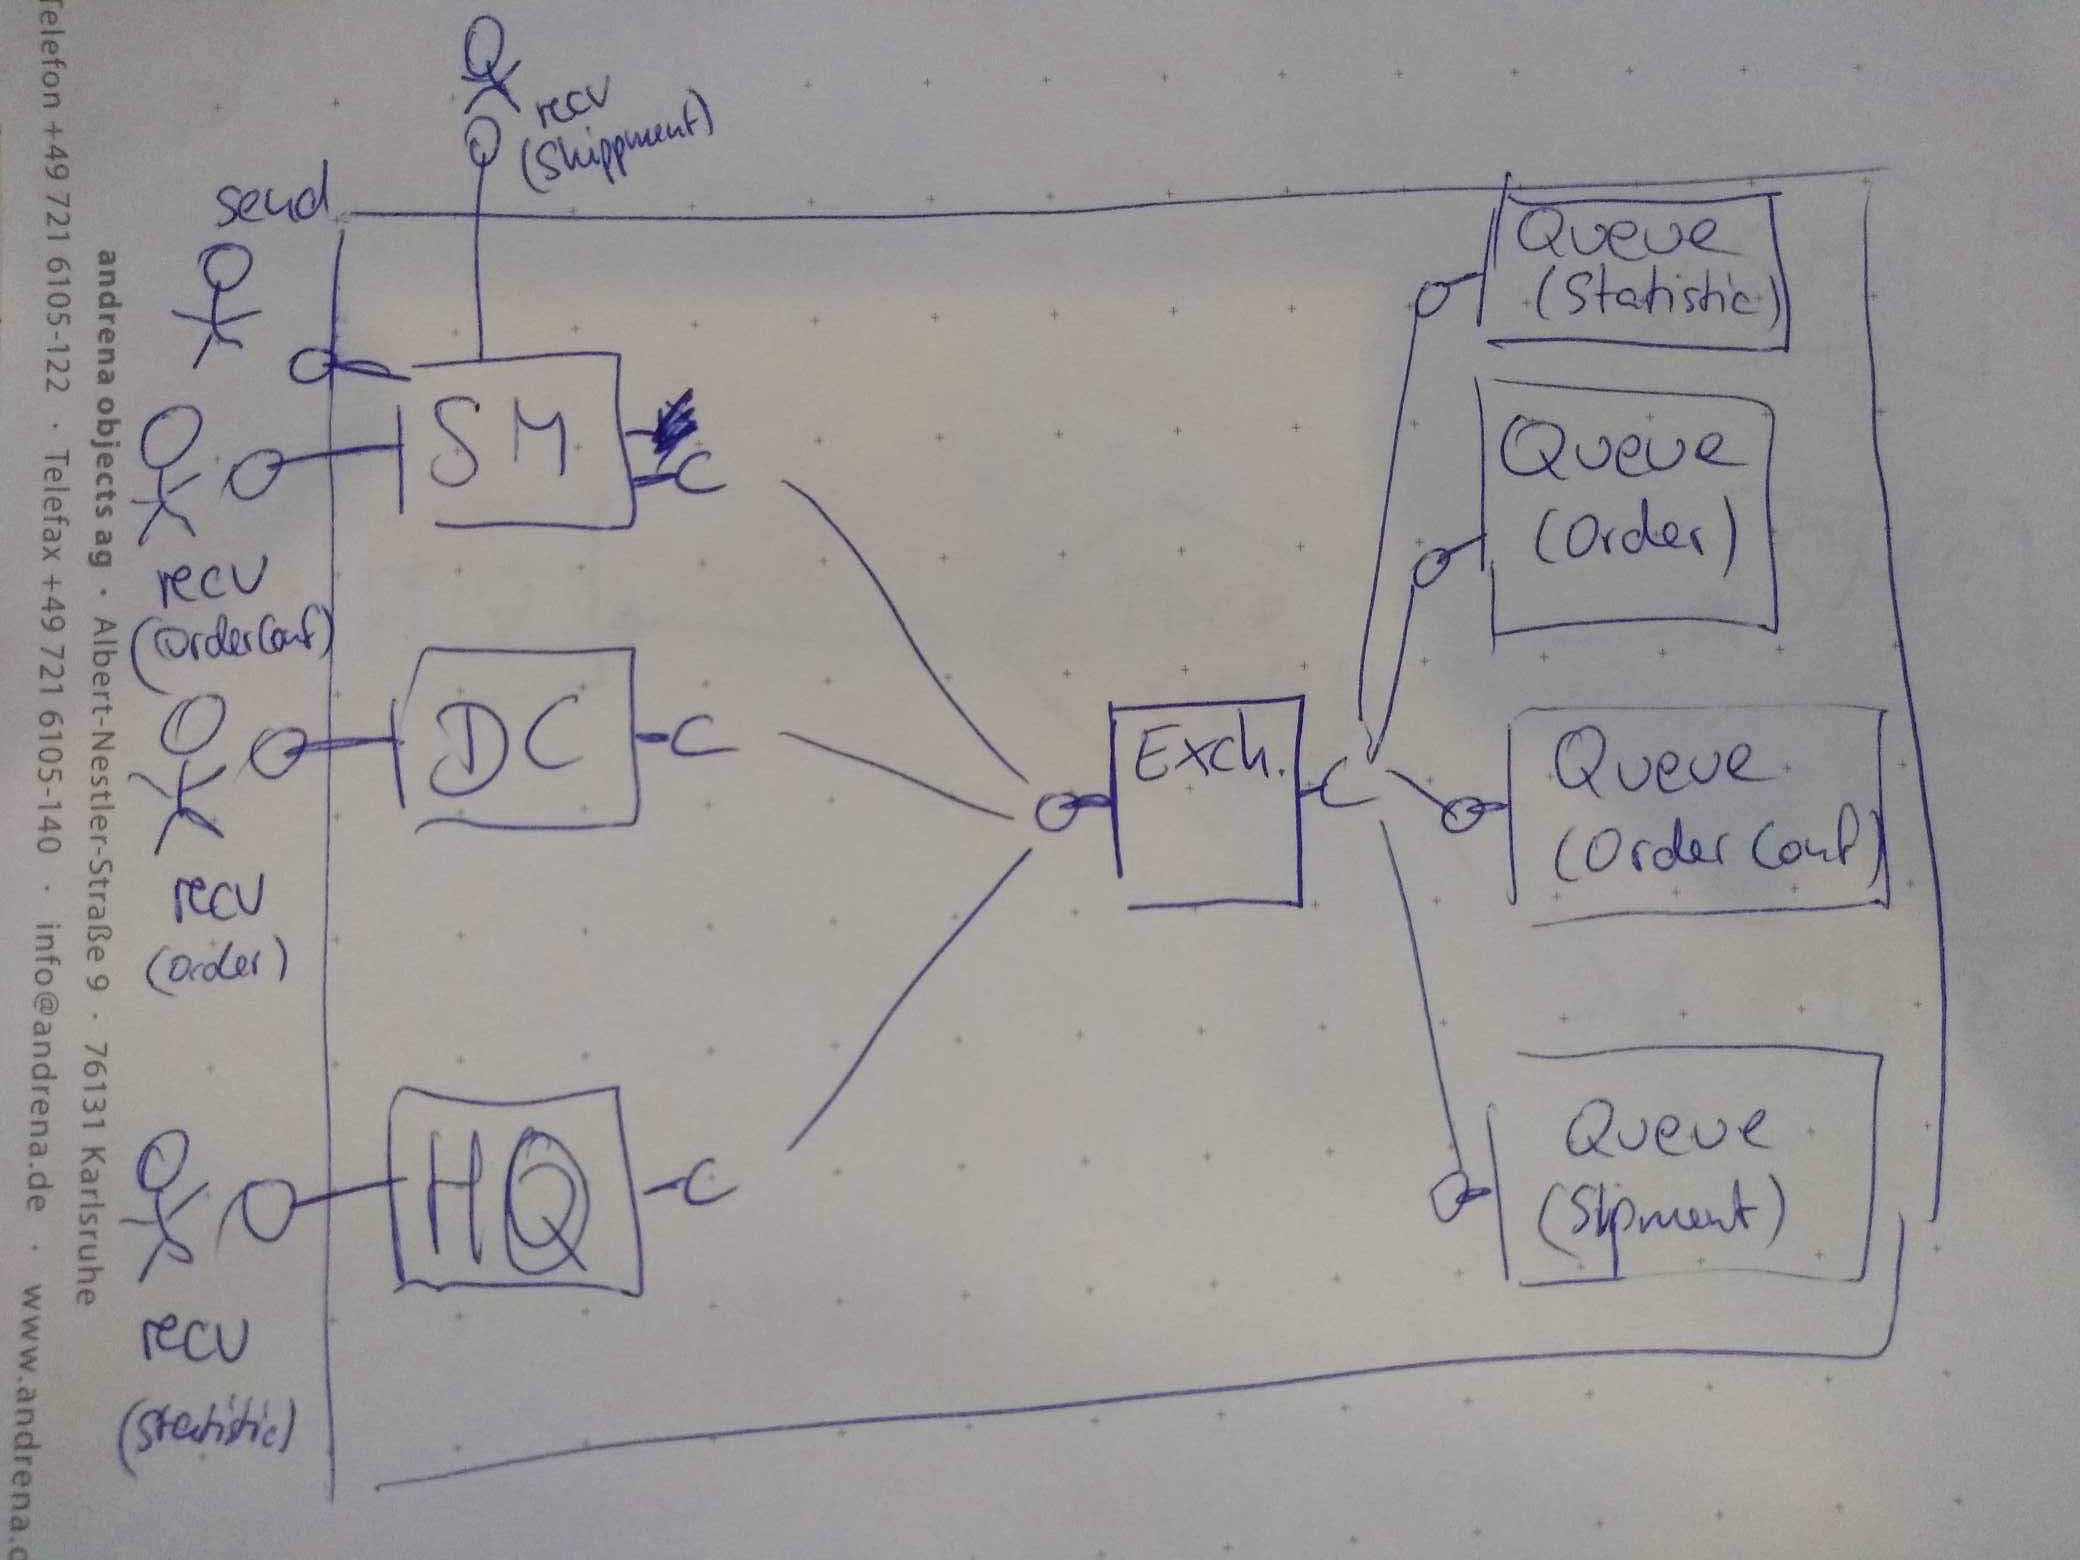
\includegraphics[width=1\textwidth]{images/evaluation/specjms/interaction1system.png}
  \caption{Interaktion 1 nach Transformation}
  \label{img:interaction1systemAfterTransformation}
\end{figure}
\subsubsection{Interaktion 3}
\autoref{img:interaction3systemAfterTransformation}
\begin{figure}
\center
  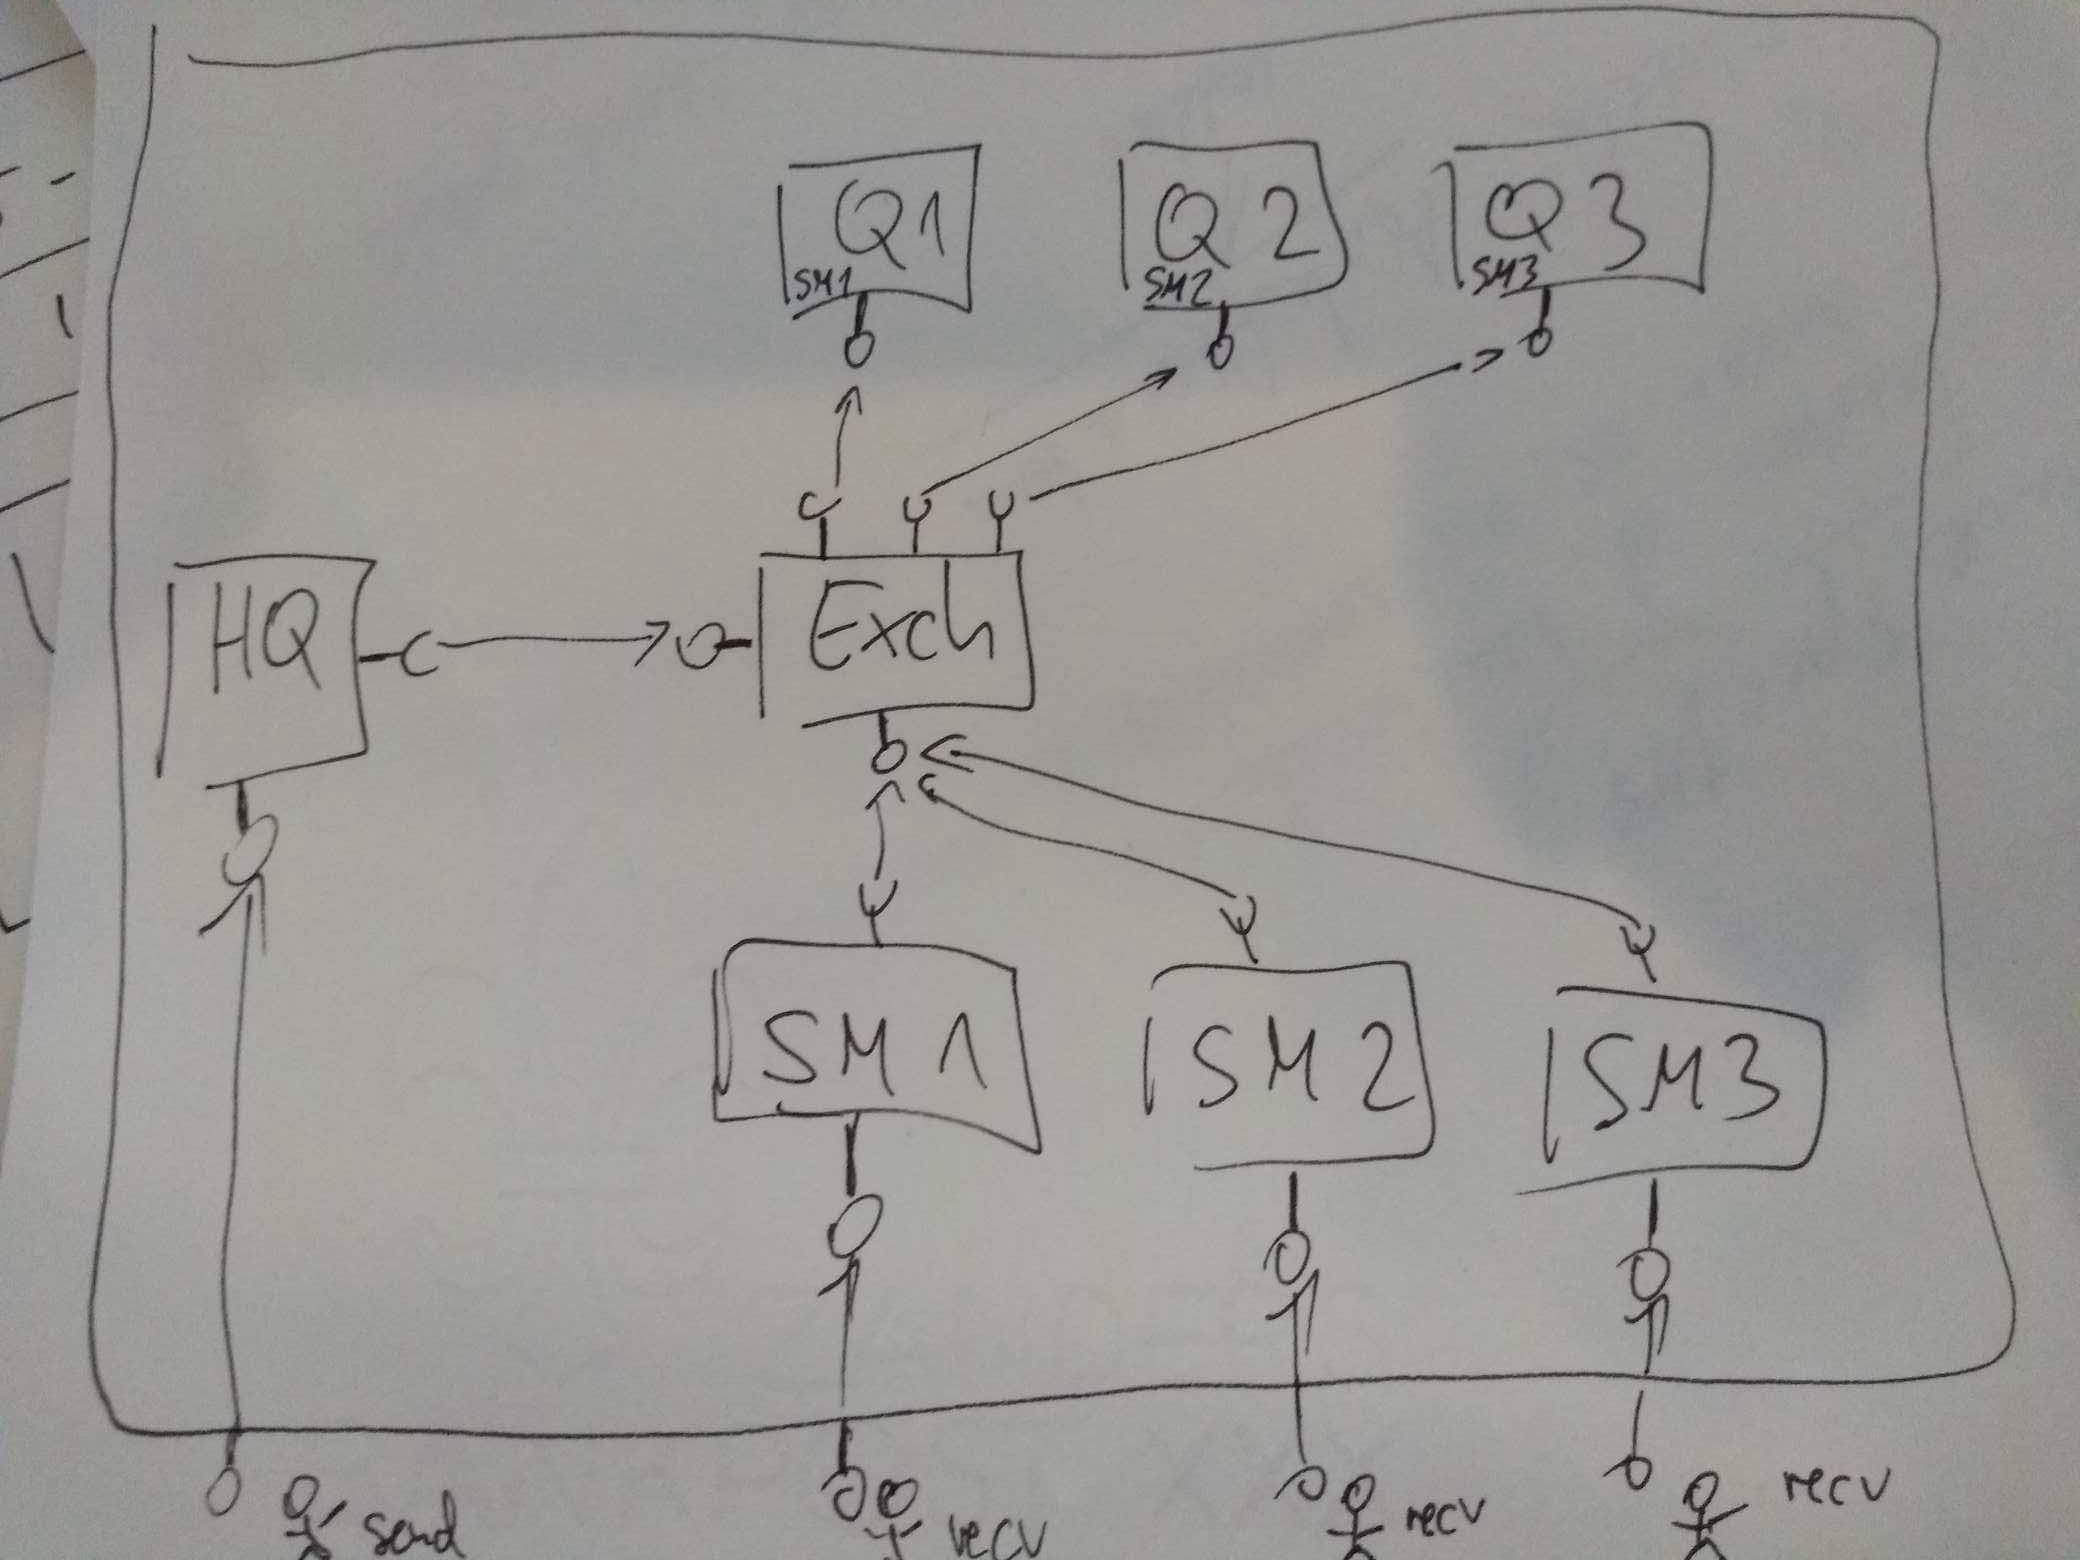
\includegraphics[width=1\textwidth]{images/evaluation/specjms/interaction3system.png}
  \caption{Interaktion 3 nach Transformation}
  \label{img:interaction3systemAfterTransformation}
\end{figure}


\section{Modell vs Implementierung}
%CPU Auslastung des Specjms vs. Modellierung\\
Fehler \% = |modell - messung| / messung * 100 \\
mehrer Messungen für Interaktion => Boxplot, der einen Median zeigt. Mit diesem wird dann das Modell verglichen.
\subsection{Interaktion 1}
evtl noch versch Groessen?
\subsubsection{Msg Rate 1}
Für diesen Vergleich wurde die Senderate der Bestellungen auf eine Bestellung die Sekunde limitiert. Im Anschluss wurde die Interaktion gestartet und nach 10 Minuten beendet. Diese Messung wurde 10 mal durchgeführt. Die durchschnittlichen Interaktionszeiten sind in \autoref{img:specjmsMsgRate1Impl} als Boxplot dargestellt. TODO Boxplot beschreiben. Die Simulation der Modellierung liefert eine Interaktionszeit von 9500 Mikrosekunden (Mit Bild?). Die Fehler sind in \autoref{tab:interaction1msgrate1error} abgebildet. Somit liegt der Fehler fuer diesen Vergleich zwischen 24.66\% und 31.21\%. 
\begin{figure}
\center
  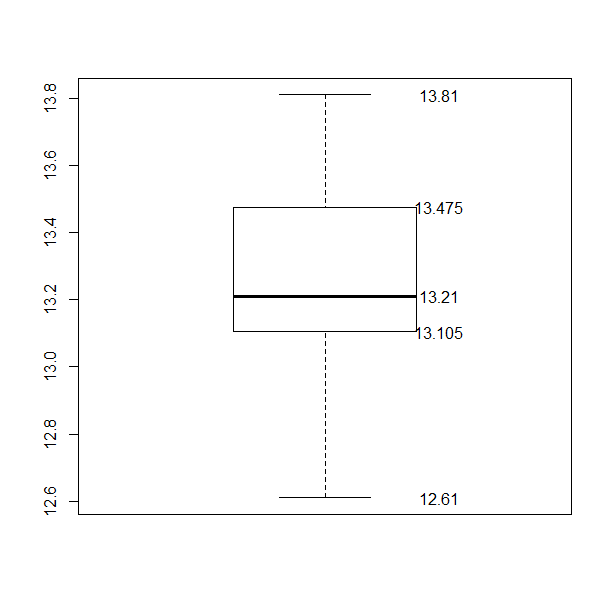
\includegraphics[width=0.6\textwidth]{images/evaluation/specjms/interaction1msgrate1.png}
  \caption{Boxplot von 10 verschiedenen Messungen der Interaktion 1}
  \label{img:specjmsMsgRate1Impl}
\end{figure}
\begin{table}
  \begin{tabular}{|l|l|l|l|l|}
    Unterer Whisker & unteres Quartil & Median & Oberes Quartil & oberer Whisker \\
    \hline
    24.66 & 26.98 & 28.03 & 29.5 & 31.21
  \end{tabular}
	\caption{\label{tab:interaction1msgrate1error} Fehler für Interaktion 1 Msgrate 1}
\end{table}
\subsubsection{Msg Rate Standard}
\subsubsection{Msg Rate Lastszenario}
Queue fuellt sich im Modell und in echt
\subsubsection{Lazy Konfiguration}

\subsection{Interaktion 3}


\section{Zusammenfassung}
Was ist das Ergebnis \\
wie ist die Genauigkeit? Besser, gleich, schlechter\\
Vergleich zu davor, auch mit Modellierungsaufwand \\

%Modellierung eroeffnet neue moeglichkeiten\\

%\section{TIME}
%Ein weiteres System, das die Anforderungen aus \autoref{sec:systemanforderungen} erfüllt, ist das Transport Information Monitoring Environment (TIME) System \cite{time}. Dabei handelt es sich um ein System der Universität Cambridge. TIME soll ein reales Verkehrsüberwachungssystem darstellen. Es besteht aus mehreren verteilten Komponenten, die verschiedene Arten von Ereignissen senden bzw. empfangen. Die standardmäßige Middleware hat eine Peer-To-Peer Architektur, Punkt-zu-Punkt Kommunikation und unterstützt asynchronen Nachrichtenaustausch. Das System überwacht Autos mithilfe von Kennzeichenerkennung und soll den Verkehrsfluss optimieren. Diese Anwendung ist interessant, weil sie Daten von verschiedenen verteilten Sensoren und Systemen sammelt und integriert. Darüber hinaus enthält es Komponenten mit hohem und unterschiedlichem Ressourcenbedarf, wie z.B. der Kennzeichenerkennungsalgorithmus. Die Systemarchitektur ist sehr anpassungsfähig, wenn es darum geht, neue Komponenten hinzuzufügen oder die Verbindungen zwischen Komponenten oder deren Standort zu ändern. Was dazu führt, dass das hinzufügen und austauschen von verschiedenen MOMs möglich ist. Für die Masterarbeit liegt sowohl die Implementierung, als auch eine PCM-Modellierung des TIME Systems aus einer früheren Arbeit von Christoph Rathfelder \cite{Rathfelder2013} vor. Das TIME System soll für diese Masterarbeit als Evaluierungssystem dienen. Die Modellierung/Implementierung soll zunächst als Referenz für die Performanzanalyse dienen und im nächsten Schritt um verschiedene MOMs erweitert werden.